\chapter{Análise Teórica}

Esta prática de laboratório é dividida em três etapas principais. A primeira consiste na análise teórica do circuito divisor de tensão e do buffer de corrente para obter os equivalentes de Thévenin. A segunda etapa foca na montagem dos circuitos e na coleta de dados experimentais em laboratório. Por fim, a terceira etapa envolve a análise dos dados coletados para estimar os parâmetros de Thévenin utilizando o MMEQ. Para os cálculos e manipulação de equações, foi utilizada a ferramenta de computação simbólica \cite{maxima}.

\section{O \textit{Buffer} de Corrente}

O \textit{buffer} de corrente é um circuito que permite transferir uma tensão de uma fonte com alta impedância interna para uma carga sem perda significativa de tensão. A configuração básica utiliza um amplificador operacional na configuração não-inversora com realimentação direta (ganho unitário), conforme mostrado na Figura \ref{fig:buffer_basico}.

\begin{figure}[H]
    \centering
    \caption{Configuração básica do \textit{buffer} de corrente com amplificador operacional.}
    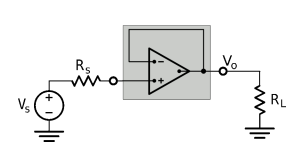
\includegraphics[width=0.5\linewidth]{FIGURAS/buffer_basico.png}
    \label{fig:buffer_basico}
    \legend{Fonte: Esquema do circuito da prática.}
\end{figure}

Para o amplificador operacional ideal, as características fundamentais são:
\begin{itemize}
    \item Resistência de entrada infinita: $R_{in} \to \infty$ (não há corrente nos terminais de entrada);
    \item Ganho de tensão infinito: $A \to \infty$;
    \item Diferença de tensão entre as entradas: $V^+ - V^- = 0$ (para ganho infinito e saída finita).
\end{itemize}

\section{Equivalente de Thévenin do Divisor de Tensão}

O circuito divisor de tensão alimentado por fontes simétricas é mostrado na Figura \ref{fig:divisor_tensao}.

\begin{figure}[H]
    \centering
    \caption{Circuito divisor de tensão com fontes simétricas.}
    \includegraphics[width=0.5\linewidth]{FIGURAS/divisor_tensao.png}
    \label{fig:divisor_tensao}
    \legend{Fonte: Esquema do circuito da prática.}
\end{figure}

\subsection{Tensão de Thévenin}

A corrente que circula pelo divisor de tensão é dada por:

\begin{equation}
    I = \frac{V_{CC} - (-V_{EE})}{R_1 + R_2} = \frac{V_{CC} + V_{EE}}{R_1 + R_2}.
    \label{eq:corrente_divisor}
\end{equation}

A tensão de saída em circuito aberto (tensão de Thévenin) é obtida aplicando-se a Lei de Kirchhoff das Tensões:

\begin{equation}
    V_{th} = -V_{EE} + I \cdot R_2 = -V_{EE} + \frac{R_2(V_{CC} + V_{EE})}{R_1 + R_2}.
    \label{eq:vth_divisor}
\end{equation}

Simplificando:

\begin{equation}
    V_{th} = \frac{R_2 \cdot V_{CC} + R_2 \cdot V_{EE} - V_{EE}(R_1 + R_2)}{R_1 + R_2} = \frac{R_2 \cdot V_{CC} - R_1 \cdot V_{EE}}{R_1 + R_2}.
    \label{eq:vth_simplificada}
\end{equation}

Para fontes simétricas ($V_{CC} = V_{EE} = V_s$):

\begin{equation}
    V_{th} = \frac{R_2 - R_1}{R_1 + R_2} \cdot V_s.
    \label{eq:vth_simetrica}
\end{equation}

\subsection{Resistência de Thévenin}

Para determinar a resistência de Thévenin, curto-circuitam-se as fontes de tensão independentes. O circuito resultante mostra $R_1$ e $R_2$ em paralelo:

\begin{equation}
    R_{th} = \frac{R_1 \cdot R_2}{R_1 + R_2}.
    \label{eq:rth_divisor}
\end{equation}

\section{Análise do \textit{Buffer} de Corrente}

O circuito completo com o \textit{buffer} de corrente é mostrado na Figura \ref{fig:circuito_completo}.

\begin{figure}[H]
    \centering
    \caption{Circuito completo: divisor de tensão seguido de buffer de corrente.}
    \includegraphics[width=0.7\linewidth]{FIGURAS/circuito_completo.png}
    \label{fig:circuito_completo}
    \legend{Fonte: Esquema do circuito da prática.}
\end{figure}

\subsection{Ganho de Tensão do \textit{Buffer}}

Utilizando análise nodal no circuito do \textit{buffer} com o modelo do ampop incluindo resistência de saída $R_o$, e considerando que:
\begin{itemize}
    \item A entrada não-inversora está conectada à fonte $V_s$ (tensão de Thévenin do divisor);
    \item A saída está realimentada diretamente para a entrada inversora;
    \item A corrente de carga é $I_L = V_o/R_L$.
\end{itemize}

O ganho de tensão do \textit{buffer} é dado por:

\begin{equation}
    A_v = \frac{V_o}{V_s} = \frac{A}{1 + \frac{R_o}{R_L}(A+1)}.
    \label{eq:ganho_buffer}
\end{equation}

Tomando o limite quando $A \to \infty$:

\begin{equation}
    \lim_{A \to \infty} A_v = \lim_{A \to \infty} \frac{A}{1 + \frac{R_o}{R_L}(A+1)} = 1.
    \label{eq:ganho_buffer_ideal}
\end{equation}

Portanto, o \textit{buffer} de corrente ideal possui **ganho de tensão unitário**.

\subsection{Equivalente de Thévenin do Buffer}

Para o \textit{buffer} de corrente ideal ($A \to \infty$), o equivalente de Thévenin apresenta:

\textbf{Tensão de Thévenin:}
\begin{equation}
    V_{th,buffer} = V_{th,divisor} = \frac{R_2 \cdot V_{CC} - R_1 \cdot V_{EE}}{R_1 + R_2}.
    \label{eq:vth_buffer}
\end{equation}

\textbf{Resistência de Thévenin:}
\begin{equation}
    R_{th,buffer} \approx 0~\Omega.
    \label{eq:rth_buffer}
\end{equation}

A resistência de Thévenin do \textit{buffer} é idealmente zero, o que significa que a tensão de saída permanece constante independentemente da carga conectada.

\section{Exemplo Numérico}

Considere o circuito com os seguintes valores:
\begin{itemize}
    \item $V_{CC} = V_{EE} = 10$~V
    \item $R_1 = 3{,}9$~k$\Omega$
    \item $R_2 = 6{,}8$~k$\Omega$
    \item $R_o = 50$~$\Omega$ (resistência de saída do ampop)
\end{itemize}

\subsection{Divisor de Tensão}

Utilizando as Equações \ref{eq:vth_simplificada} e \ref{eq:rth_divisor}:

\begin{equation}
    V_{th} = \frac{6{,}8 \times 10 - 3{,}9 \times 10}{3{,}9 + 6{,}8} = \frac{29}{10{,}7} = 2{,}710~\text{V}.
\end{equation}

\begin{equation}
    R_{th} = \frac{3{,}9 \times 6{,}8}{3{,}9 + 6{,}8} = \frac{26{,}52}{10{,}7} = 2{,}479~\text{k}\Omega.
\end{equation}

\subsection{\textit{Buffer} de Corrente}

Para o \textit{Buffer} ideal conectado ao divisor:

\begin{equation}
    V_{th,buffer} = 2{,}710~\text{V}.
\end{equation}

\begin{equation}
    R_{th,buffer} \approx 0~\Omega.
\end{equation}

Os valores calculados estão sumarizados na Tabela \ref{tab:valores_teoricos}.

\begin{table}[H]
    \centering
    \ABNTEXfontereduzida
    \caption{Valores teóricos dos equivalentes de Thévenin.}
    \label{tab:valores_teoricos}
    \begin{tabular}{l|c|c}
        \hline
        \textbf{Circuito} & \textbf{$V_{th}$ (V)} & \textbf{$R_{th}$ (k$\Omega$)} \\ \hline
        Divisor de Tensão & 2,710 & 2,479 \\ [3pt]
        Divisor + \textit{Buffer} & 2,710 & $\approx 0$ \\ [3pt]
        \hline
    \end{tabular}
    \legend{Fonte: Elaborado pelos autores.}
\end{table}

Estes valores teóricos servirão como referência para comparação com as medições experimentais e estimativas pelo MMEQ realizadas nas etapas subsequentes.